\section{Metodología}\label{sec:metodologia}

A la hora de gestionar un proyecto, es recomendable definir una metodología de
trabajo, seguimiento y control con el fin de asegurar el correcto cumplimiento y
finalización de su lista de requisitos y objetivos. Tras investigar y plantear
distintas alternativas, se ha escogido la metodología Kanban para desarrollar
este proyecto.

El método Kanban como tal es útil si se desea:
\begin{itemize}
    \item Iniciar un proyecto de manera ágil, rápida, de coste nulo y bajo riesgo. % Getting off to a low-risk, zero-cost, agile, fast start.
    \item Analizar y mejorar el proceso de trabajo ya existente. % Pinning down existing workflows and spotting glaring errors.
    \item Controlar múltiples grupos de tareas. % Controlling multiple pieces of unconnected work.
    \item Asegurar que el número de tareas en ejecución están dentro de un nivel aceptable. % Keeping the numbers of jobs in play down to an acceptable level.
    \item Cambiar a una mentalidad de desarrollo ágil. % Getting the team into an agile way of thinking.
\end{itemize}

Esta sección, por tanto, estará dedicada a explicar los conceptos e ideas
necesarias de cara a justificar la razón por la cual se ha escogido este método
de trabajo. Además, es necesario mencionar que esta información será resumida
principalmente de \cite{Cole2015-fd} y \cite{Stellman2014-qr}, siendo éstas las
referencias recomendadas en caso de desear más detalles al respecto.
\subsection{Definición}

El método Kanban tiene sus orígenes en las fábricas de coches de Toyota a manos
de Taiichi Ohno. Fue creado como un simple sistema de planificación y
administración de trabajo e inventario de cada fase de producción. Sin embargo,
fue David J. Anderson quien definió y adaptó esta metodología para el uso en
ingeniería y desarrollo de software.

Es necesario mencionar que, contrario a lo que se piensa normalmente, Kanban es
una metodología ágil de mejora de procesos y no un framework de administración
de proyectos. Y así como muchos métodos de este tipo, se caracteriza
principalmente por ser evolutivo e iterativo en el tiempo.

Asimismo, Kanban comparte la misma ideología de trabajo con el método Lean hasta
tal punto que se considera que es una especialización de esta última. Aplicando
los principios y valores de este proceso, Kanban se centra en eliminar los
desperdicios de tiempo y recursos que el equipo tiene. Por lo tanto, este
proceso de mejora pide a los equipos de desarrollo empezar con una metodología
ya existente para poder perfeccionarla gradualmente en el tiempo a través de la
experimentación, el cálculo de distintas métricas de rendimiendo y la
confirmación de resultados positivos según dichas medidas.

Todo equipo cuenta con un sistema para la implementación de código, ya sea que
se siga una metodología formal como Scrum o que se disponga de una serie de
reglas no definidas o reconocidas explícitamente. Como consecuencia de esto, lo
único que se necesita para empezar a utilizar Kanban es identificar el proceso
de desarrollo actual para poder formalizarlo y adaptarlo a esta metodología.

Por tanto, aunque Kanban no es un sistema de gestión de proyectos, es posible
hacer uso de éste para ello al tener como principal objetivo aumentar la
predictabilidad del flujo de trabajo y así mejorar la planificación del proyecto
como tal.

\subsection{Principios de Kanban}
Al ser una especialización del método Lean, se tiene una serie de principios
directores en esta metodología. Especificamente se pueden listar los siguientes
tres:
\begin{itemize}
    \item \textbf{Empieza con lo que se hace actualmente}: %Start with what you do now
    Como se había mencionado anteriormente, el método Kanban pide requiere de un
    proceso o metodología inicial. Es a través del análisis y la comprensión de
    dicho proceso que Kanban permite perfeccionarlo iterativamente. Pero como
    consecuencia de esto, no es posible aplicar Kanban adecuadamente si se
    desconoce la metodología que usa el equipo de desarrollo.

    \item \textbf{Comprométete al cambio evolutivo e incremental}: %Agree to pursue incremental, evolutionary change
    Aunque parezca muy repetitivo, es necesario volver a mencionar que el
    objetivo de Kanban es la mejora gradual del sistema. A eso se refiere el
    cambio evolutivo e incremental y es por eso que el método pide calcular
    métricas de control. Es a través de estas medidas que se llegan a conocer
    las partes mejores del proceso de desarrollo.

    \item \textbf{Respeta el proceso, los roles, las responsabilidades y títulos
    actuales}: %Respect the current process, roles, responsibilities and titles
    Cuando el equipo de trabajo dedica tiempo a medir el rendimiento del
    sistema, es posible encontrar ciclos de retroalimentación que contienen
    información importante para la mejora evolutiva del proceso. Sin embargo,
    para poder aplicar dicha información es necesario conocer cómo se aplica
    ésta a cada rol del equipo. Por esta razón Kanban considera relevante
    respetar las responsabilidades y roles asociadas a cada miembro del grupo.
\end{itemize}

\subsection{Prácticas de Kanban}

El método Kanban, además, define explícitamente una serie de prácticas a llevar
a cabo con el fin de aplicar correctamente la mejora de procesos que éste
permite. Sin embargo, no es necesario hacer uso de todas estas en su totalidad
al iniciar con el método. Kanban tiene específicamente los siguientes seis principios:

\begin{itemize}
    \item \textbf{Definir y visualizar el flujo de trabajo}: %Define and Visualise Workflow
    Con el fin de familiarizarse más con el proceso de trabajo, Kanban pide
    hacer uso de representaciones visuales de éste a través de tablones, listas
    de trabajo y elementos de trabajo. La combinación de dichos componentes
    permite definir el flujo de trabajo en su totalidad de una manera fácilmente
    entendible. En Kanban, visualizar significa anotar exactamente lo que hace
    el equipo sin embellecer los detalles con el fin de observar el sistema en
    su totalidad.

    \item \textbf{Limitar el trabajo en progreso}: %Limit work-in-progress
    En el método Kanban los distintos trabajos a realizar en el proceso de
    desarrollo tienen un límite de tareas en ejecución en un determinado
    momento. La justificación que se le da a este principio recae en el hecho de
    que realizar múltiples labores a la vez reduce la eficiencia del equipo. A
    dicho límite se le conoce como \emph{WiP} (de sus siglas en inglés
    \emph{Work-in-Progress}) o \emph{Trabajo en Progreso}.

    \item \textbf{Manejar el flujo de trabajo}: %Manage the flow of work
    Una vez definido el flujo de trabajo, el objetivo será conseguir una rápida
    y suave transición entre los distintos grupos de tareas, desde la lista de
    trabajo a empezar hasta dar por finalizada la labor. Si se consigue esta
    velocidad de flujo, se dice que se está operando con la eficiencia óptima y
    es en este momento que se crea el máximo valor laboral en el menor tiempo
    posible. A medida que el equipo desarrolla, se van encontrando los cuellos
    de botella y ajustando los límites de trabajo.

    \item \textbf{Hacer explícitas las políticas de proceso}: %Make the process explicit
    Para poder obtener un flujo de trabajo óptimo, además, es necesario definir
    los objetivos que se deben cumplir para dar por terminada una serie de
    tareas con el fin de determinar cuándo se avanza de estado. Dichas
    condiciones de finalización, sin embargo, siempre irán ligadas al tipo de
    proceso que se está utilizando y, por tanto, deberán ser discutidas y
    especificadas por el equipo.

    \item \textbf{Implementar ciclos de retroalimentación}: %Implement Feedback Loops
    Como se había mencionado anteriormente, los ciclos de retroalimentación
    permiten identificar la información necesaria para aplicar mejoras en el
    proceso de desarrollo. Kanban define dichos ciclos como la combinación de
    limitaciones que permiten dar a conocer los puntos débiles del equipo y su
    correcta implementación requiere de experimentación y análisis del
    rendimiento general del sistema.

    \item \textbf{Mejorar colaborativamente}: %Improve collaboratively
    Una vez que Kanban ya está implementado y el foco de atención recae en el
    flujo de trabajo, el carácter de mejora incremental del método vuelve a
    salir a la luz. Es a través de la discusión, análisis y puesta en marcha de
    nuevas ideas que el equipo puede encontrar bloqueos en el proceso y
    adaptarse a cambios rápidamente.
\end{itemize}

\subsection{Herramientas de Kanban}

Para poder hacer uso de los principios y aplicar correctamente las prácticas del
método, existen una serie de herramientas y artefactos comunes dentro de la
metodología Kanban.

\begin{figure}[H]
    \centering
    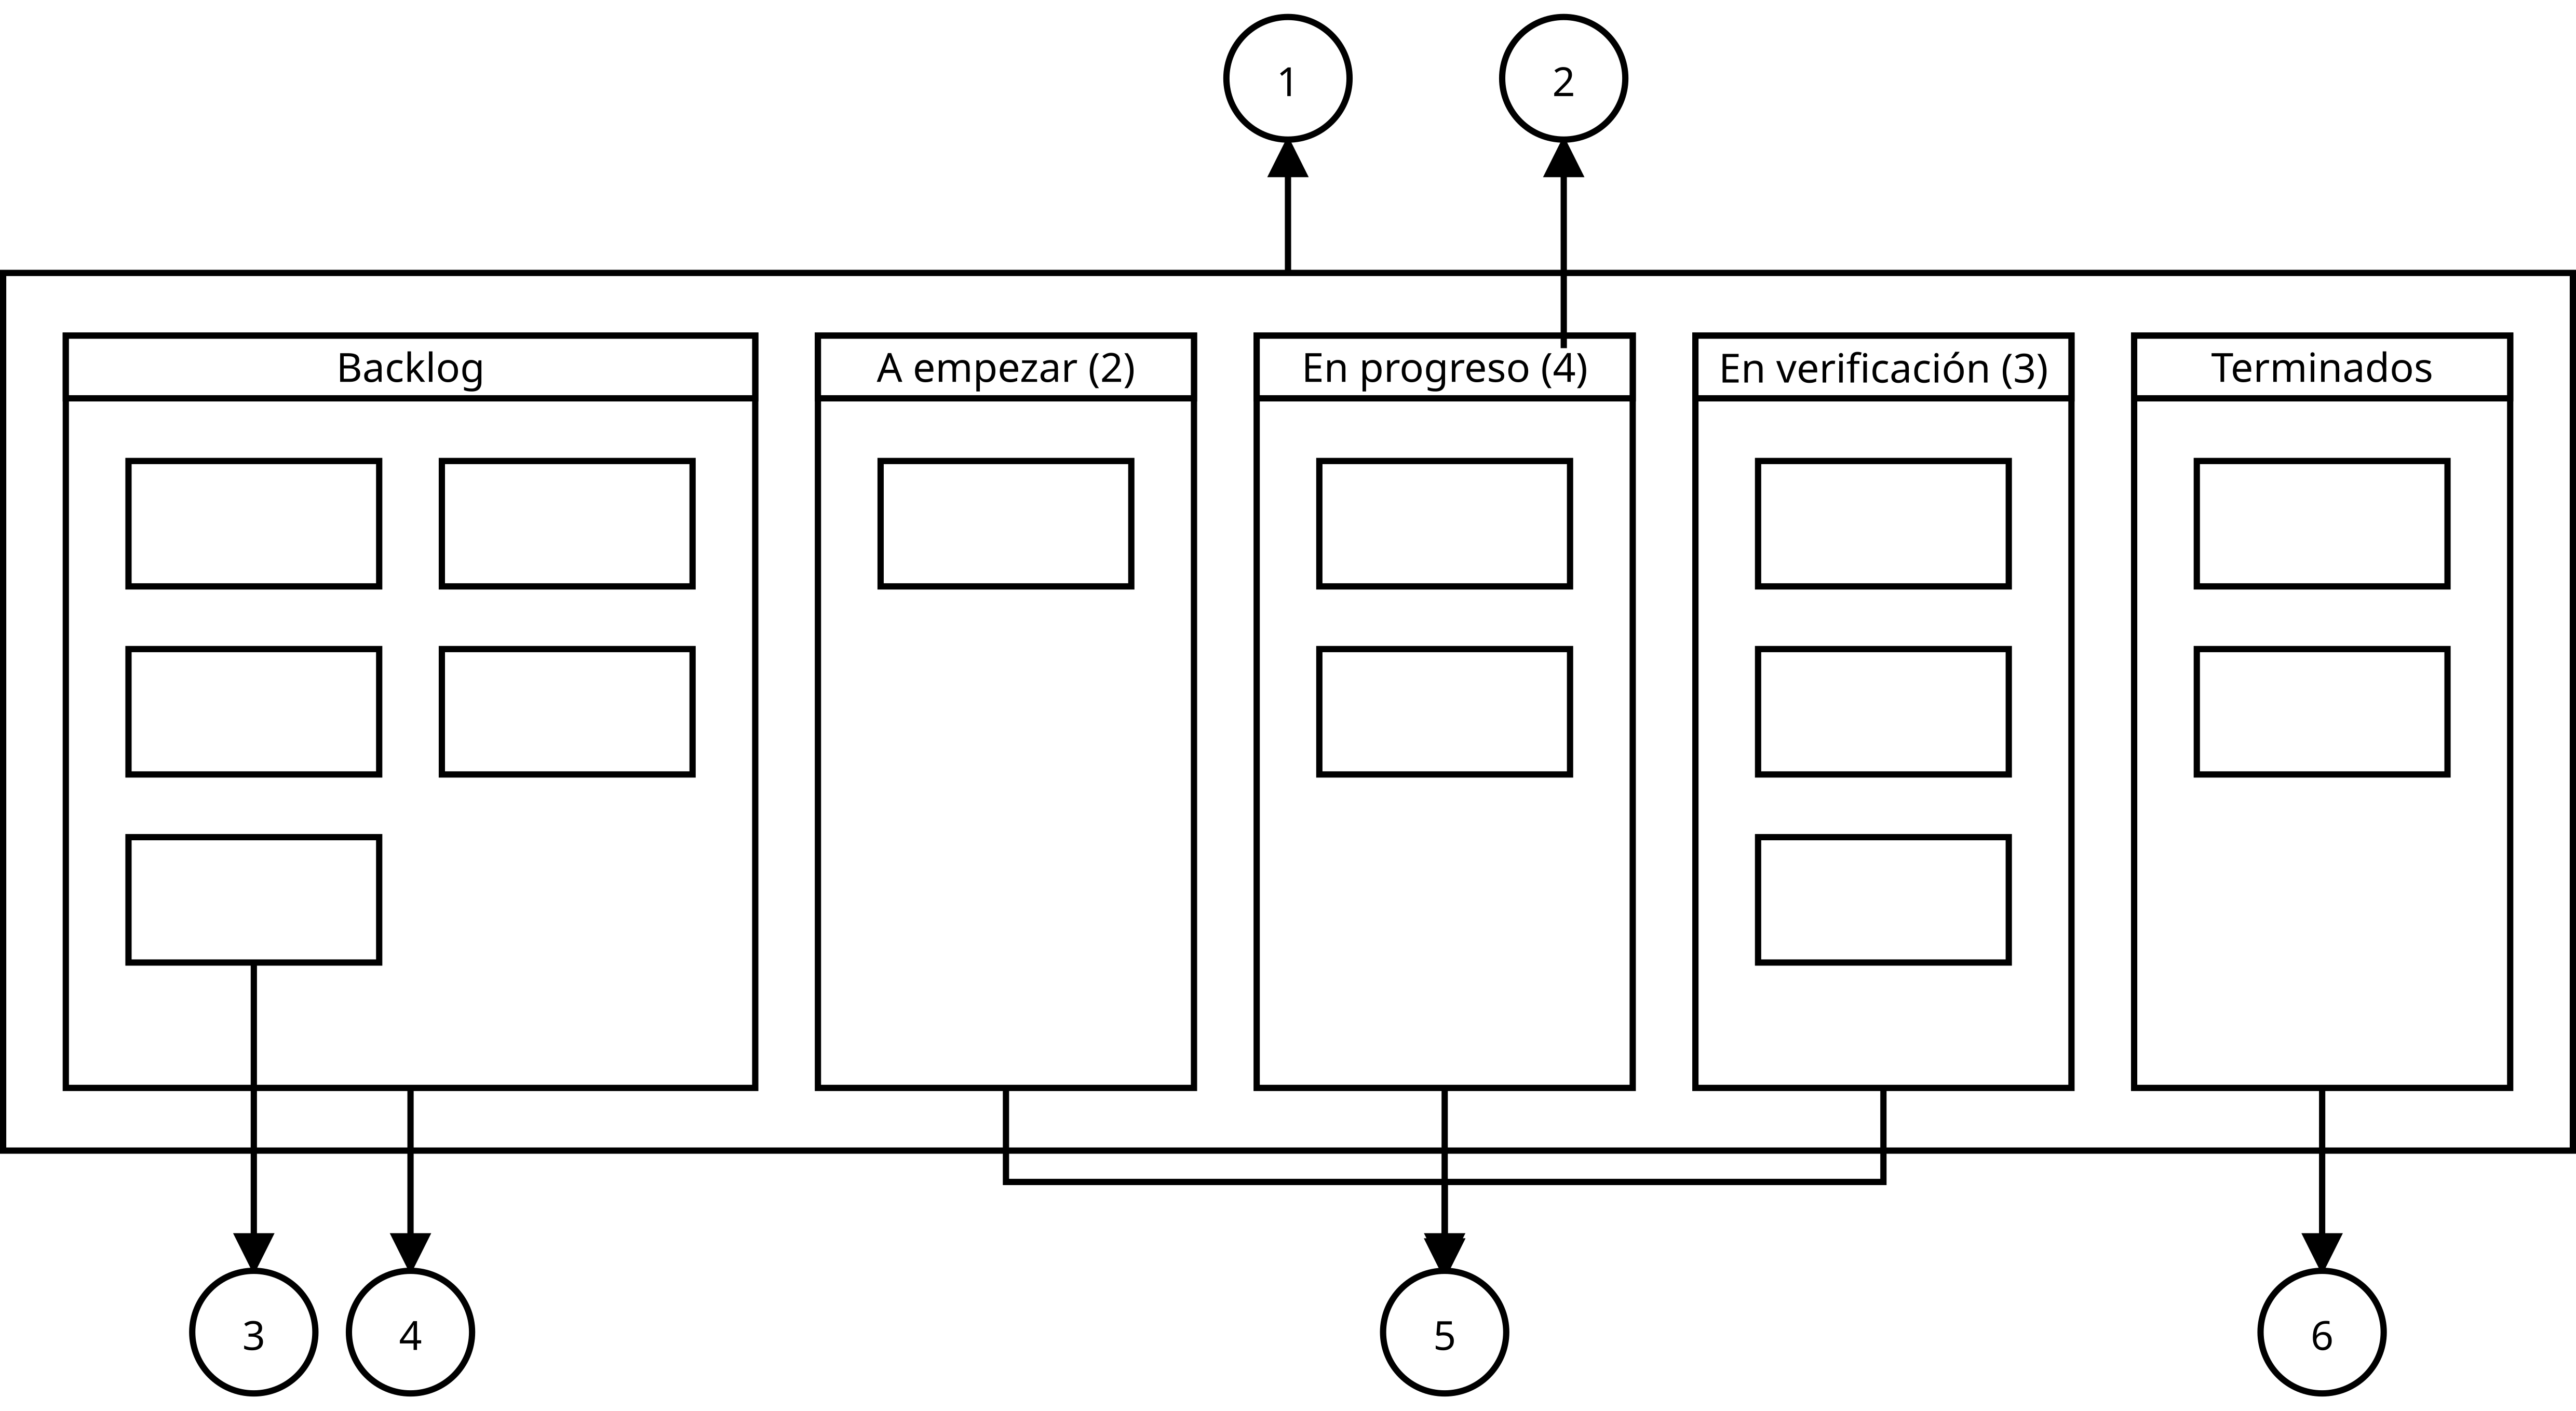
\includegraphics[width=0.85\linewidth]{5-Cuerpo/Chapter2/TablonKanban.png}
    \caption{Ejemplo de un tablón kanban}
    \label{fig:kanbanboard}
\end{figure}
\improvement{INSERTAR UNA IMAGEN DE UN TABLÓN KANBAN COMPLETO}

Como se puede observar en la figura \ref{fig:kanbanboard}, muchos de los elementos visibles ya
habían sido referenciados anteriormente. Sin embargo, se procederá a dar una
explicación detallada de lo que representan y qué rol cumplen:

\begin{itemize}
    \item \textbf{Tablón}: % kanban board
    Como núcleo de la visualización del proceso está el tablón kanban (nótese la
    diferencia en la capitalización del nombre). Dichos tablones contienen las
    listas de tareas a realizar y permiten observar el flujo de trabajo del
    equipo a través de columnas y cartas. Cada grupo deberá especificar su
    propio tablón kanban en función de su proceso de desarrollo y es a través de
    éste que se podrán calcular las métricas, encontrar los ciclos de
    retroalimentación y determinar qué se debe mejorar para maximizar la
    eficiencia. En la figura \ref{fig:kanbanboard} está representado por el
    elemento $1$.

    \item \textbf{Listas o Columnas}:
    Para poder visualizar correctamente el flujo de trabajo dentro del tablón
    kanban se hacen uso de listas de tareas o columnas. Dichos elementos
    representarán los pasos que debe seguir una tarea para pasar por todo el
    flujo desde que se plantea como labor hasta que se finaliza. En el método se
    dice que las tareas son \emph{tiradas} (\emph{pulled} en inglés) a la
    siguiente lista una vez que se cumplen las condiciones de finalización de la
    columna en la que se encuentra. Entre los tipos de columnas que se pueden
    encontrar están:
    \begin{itemize}
        \item \textbf{Backlog}: Contiene la lista de tareas que se plantean
        realizar, pero aún no se han empezado o que pueden terminar siendo
        descartados. Éstas son las ideas de lo que se quiere desarrollar, pero
        que aún no se han materializado en labor. Dichos elementos deberán estar
        enfocados a contribuir con los objetivos del producto a implementar. En
        la figura \ref{fig:kanbanboard} está representada por el elemento $4$.
        \item \textbf{Listas intermedias}: El tablón kanban, al depender mucho
        proceso del equipo y no poder ser estandarizado, hará uso también de
        distintas columnas intermedias entre el \emph{backlog} y la columna de
        tareas finalizadas. Dichas listas serán representativas del flujo de
        trabajo que sigue el grupo como tal para desarrollar el proyecto.
        Tipicamente se pueden encontrar columnas como: \emph{a diseñar}, \emph{a
        empezar}, \emph{en progreso}, \emph{en verificación}, entre otras. En la
        figura \ref{fig:kanbanboard} están representadas por el elemento $5$.
        \item \textbf{Terminado}: Contiene la lista de tareas que se han dado
        por finalizadas en su totalidad. Esta columna es la última del tablón
        para el equipo y aquí es donde estarán todas las tareas completadas una
        vez que han pasado por todo el flujo de desarrollo. En la figura
        \ref{fig:kanbanboard} está representada por el elemento $6$.
    \end{itemize}

    \item \textbf{WiP}: Con el fin de aplicar las prácticas de limitación y
    manejo del flujo de trabajo, a cada columna se le asigna un límite de tareas
    que puede contener en un determinado momento. Si dicha lista llega a su
    límite, no se podrán traer tareas a ella hasta que se liberé de los labores
    que contiene. Normalmente dicho límite se escribe al lado del nombre de su
    respectiva columna. En la figura \ref{fig:kanbanboard} está representado por el
    elemento $2$.

    \item \textbf{Cartas}:
    Así como el tablón kanban contiene listas de trabajo, dichas columnas
    también contienen unos elementos conocidos como \emph{cartas}. Éstas
    representan las actividades y trabajos a realizar con el fin de avanzar con
    proyecto, siempre teniendo en cuenta que dichos elementos deben aumentar el
    valor del producto y tienen que ser significados para su finalización. En la
    figura \ref{fig:kanbanboard} están representadas por el elemento $3$.
\end{itemize}

\subsection{Métricas de flujo}
Para finalizar con el contenido teórico del método, se hablarán de las distintas
métricas que se utilizan para determinar la eficiencia del proceso y los
elementos  a mejorar según la metodología Kanban. Daniel S. Vacanti define en
\cite{Daniel2022} la siguiente lista de medidas:

\begin{itemize}
    \item \textbf{Trabajo en progreso}: Es el número de elementos o cartas de
    trabajo iniciados pero no finalizados.
    \item \textbf{Rendimiento}: Es el número de elementos de trabajo finalizados
    por unidad de tiempo.
    \item \textbf{Edad del elemento de trabajo}: Es el tiempo transcurrido desde
    que se inició el trabajo hasta el momento actual.
    \item \textbf{Tiempo de ciclo}: Es la cantidad de tiempo transcurrido desde
    que se inicia un trabajo y se termina.
\end{itemize}

\subsection{Justificación de la metodología}

\begin{markdown}
* No se puede realizar una estimación de las tareas ni dedicaciones a priori.
* Al ser un proyecto planteado por el estudiante, se espera mucha variabilidad
en cuanto a requisitos y entregables a lo largo del desarrollo.
* Debido a cuestiones de tiempo, la metodología debe permitir adaptarse
fácilmente a cambios en el tiempo que se le puede dedicar al proyecto.
* Debido a algunos aspectos que se desconocen en cuanto al alcance, el método a
utilizar debe permitir adaptarse rápidamente a la integración de nuevo
conocimiento.
* El proyecto se caracteriza, entonces, por su alto nivel de desconocimiento y
variabilidad en cuanto a requisitos, objetivos y supuestos. Se tiene que lo
mejor es un desarrollo iterativo y ágil.

\end{markdown}


% -----------------------------------------------------------------------------

\subsection{Adaptación de la metodología}\label{subsec:kanban_adaptacion}
\urgent[inline]{Redacción rápida e introductoria a esta subsección}

\change[inline]{
Once the starting format of the Kanban board is agreed, the
first and almost pivotal decision to be made is whether to go for
a physical board or an electronic one. Both have their pros and
cons and there may be working practices that guide the final
decision. A virtual board can't be beaten for accessibility and
ease of sharing, as you're never more than a smart phone or
iPad away. But in our opinion the most important thing is for
the board to be highly visible, and nothing can beat a physical
board for that.
A high-profile, physical board has an almost magical quality, like
a fireplace in a huge front room, and draws people in. To start
with it's more about curiosity, yet after a short while it becomes
a centrepiece and focus for team activities. Work is planned,
prioritised and progressed around the board. A physical board
is also guaranteed to generate huge interest in unlikely places.
Senior management love the visibility of a board, so expect a
visit from the CEO or Finance Director within a week. For
once they'll see what's really going on in the organisation
without quizzing middle management or ploughing through
turgid weekly reports.
Despite our absolute preference for an old-fashioned physical
board, there are times when an electronic board either makes
more sense or is even the only viable option. When individuals
are regularly on the move or if the team is split over different
locations, there are insurmountable physical issues to deal with
and a tech option become more attractive.
But before giving up on having a physical board think carefully,
especially when trialling agile for the first time. A tech alternative
will work well enough from a functional perspective but is far
less visible and engaging, so many soft benefits will be lost.
Don't go down that route just because members of the team
occasionally work from home. Don't throw the baby out with
the bathwater.
If an electronic board is the only workable solution, consider
driving it from a physical source - start with a wall and duplicate.
The overhead of keeping two boards in sync will be offset by the
benefits of having a real board. But when all else fails there are
plenty of electronic options with good coverage across the main
devices. Some are completely free and all the rest offer a trial
period, so try before you buy.
}

Se sacará la información de aquí: \cite{Brechner2015-dv} % Teoría aplicada (el
de Xbox)

\change[inline]{Uno de los artefactos es el tablón como tal. Aquí se define Trello como tablón online/virtual}
\change[inline]{Definición de Trello y un poco de transfondo}

\subsubsection{Definir y visualizar el flujo de trabajo}
% Define aquí el tablón, las listas, las etiquetas y el formato de las cartas

% \subsubsection{El tablón kanban}
% \urgent[inline]{INSERTAR CAPTURA DEL TABLÓN}
% \subsubsection{Significado de las listas}
% \urgent{DEFINE LOS WIPS DE LAS COLUMNAS}

% \begin{itemize}
%     \item \textbf{Backlog}: La columna que contendrá la lista de tareas e ideas
%    espera de ser empezadas en la iteración.
%     \item \textbf{To Do}: Del inglés \emph{a hacer}, contiene la lista de
%     tareas cuya labor ha sido empezada en la iteración.
%     \item \textbf{Doing}: Del inglés \emph{en progreso}, contiene la lista de
%     tareas cuya labor se está realizando en la iteración.
%     \item \textbf{Testing}: Del inglés \emph{en verificación}, contiene la lista de
%     tareas cuya labor se ha finalizado pero todavía se está determinando si
%     cumplen con las condiciones de finalización para pasar a la lista de tareas
%     terminadas.
%     \item \textbf{Done}: Del inglés \emph{terminado}, contiene la lista de
%     tareas cuya labor se ha dado por terminada y que están en espera de ser
%     discutidas en la reunión de fin de iteración.
%     \item \textbf{Approved}: Del inglés \emph{aprobado}, contiene la lista de
%     tareas discutidas y cuya realización ha sido aceptada como adecuada para la
%     finalización del proyecto.
% \end{itemize}

% \subsubsection{Formato de las cartas}

% \change[inline]{Aquí se definen las cartas que son otro artefacto de Kanban. Conviene mejor usar capturas}

% %! Aquí conviene mejor una captura

% % \begin{markdown}
% %     # Ge.P-1: Definición de la metodología de gestión
% %     **Iteraciones:** 2
% %     **Código:** FeI
% %     **Tarea:** 1
% %     **Tiempo Estimado:** 0.0
% %     **Tiempo Usado:** 0.0
% %     **Desviación:** 0.0
% %     **Descripción:** nan
% % \end{markdown}

% \subsubsection{Significado de etiquetas}
% \change[inline]{Un añadido que se puede utilizar son las etiquetas como artefacto. Aquí se definen}
% \begin{itemize}
%     \item \textbf{Bug:} Cuando se detecta un error y se debe arreglar
%     \item \textbf{Bloqueado:} Cuando una tarea no se puede completar debido a
%     otras circunstancias
%     \item \textbf{Pendiente:} Abreviado de “Pendiente de Retroalimentación”.
%     Indica que esta tarea debe discutirse en una reunión
%     \item \textbf{No aceptada:} Indica que la tarea no ha sido aceptada para
%     continuar en la siguiente iteración y debe retrabajarse, cambiarse o
%     descartarse.
% \end{itemize}

\subsubsection{Limitar y manejar el trabajo en progreso}
% Definir aquí los WiPs
\subsubsection{Hacer explícitas las políticas de proceso}
% Criterios de finalización aquí

% \subsubsection{Criterios de movimiento de listas}
% \change[inline]{Se comentó que hay que definir el concepto de “finalizado” para cada lista. Aquí se hace eso}
% % Qué cosas se cumplen para que una carta se mueva a la siguiente lista. Agile Project Managament With Kanban pag. 24 (set limits on chaos and Step 4: Define done)
% % Pull Criteria

% \subsubsection{Criterios de bloqueo de tareas}

\subsubsection{Implementar ciclos de retroalimentación}
% Reuniones de fin de iteración y de replanificación
